%!TEX root = ../../dissertation.tex
%%%%%%%%%%%%%%%%%%%%%%%%%%%%%%%%%%%%%%%%%%%%%%%%%%%%%%%%%%%%%%%%%%%%%%%%%%%%%%%%
\section{Background}
\label{c3:sec:background}
%% reliable streaming
	%Web-based video streaming in general
	%Web, Flash, HTML5
	%relevance for mobile and future Internet
	%Drawbacks (no streaming, scaling, signaling, etc)
	%Internet Load and Video delivery performing with load
	%Example of YouTube
	%applicable quality metrics (normal metrics don't apply, no video quality scaling, observable only initial buffering time, stalls during playback, number, length, frequency thereof)


Before diving into the model some technical groundwork has to be laid. We describe protocols commonly used in the past and present and how to classify them. This is followed by other work related to this approach.

%%%%%%%%%%%%%%%%%%%%%%%%%%%%%%%%%%%%%%%%%%%%%%%%%%%%%%%%%%%%%%%%%%%%%%%%%%%%%%%%
\subsection{Definition} 

Any digitally stored video consists of a number of frames, organized into variable-sized groups, and audio samples which are played in sequence. Frames, single images of the video, do not only make use of typical spatial image compression mechanisms but encompass also temporal motion compensation, creating a dependence between frames. Videos can be encoded with a bit rate that is constant or variable over time. Typically, a variable bit rate encoding is chosen as these schemes offer a higher compression rate. To correctly display a frame, all previous frames in a block need to be present. 

Streaming, or to be more precise video streaming, is the process of playing a video while it is still being transmitted over a medium. As there is no need to have a file stored locally, received frames are typically put in a buffer to be played at the correct time. The amount of buffered video depends on the allocated buffer size as well as the video bit rate, and the transmission bit rate. It can also be controlled by the time offset between receiving the first frame of a video and actually playing it.


%%%%%%%%%%%%%%%%%%%%%%%%%%%%%%%%%%%%%%%%%%%%%%%%%%%%%%%%%%%%%%%%%%%%%%%%%%%%%%%%
\subsection{Streaming Classification}

Video streaming is a broad term covering a wide spectrum of applications as well as possible implementations. To break down and classify this field we define the following criteria to make a distinction.

\paragraph{Video Source}
The first criterion is the source of the video with the two major sources being a file stored on a remote server or a live source. Stored video can be streamed and played at any point in time. Live sources, on the other hand, are transmitting only at a fixed point in time. Depending on the type of content the timeliness of playback may also be important (imagine you are watching a game that is played right now).


\paragraph{Adaptivity of Content}
Video streaming can also be distinguished based on its adaptivity. In the simplest case there is no adaptivity present and the video is available in only one bit rate (which may still be a variable bit rate). 
But there are cases where an adaptation of the bit rate would be helpful. For example to accommodate for a clients needs in matters of the screen size. Usually, adaptation is used to tune the video stream to the currently available connection bandwidth. Adaptation can be achieved in two ways. Either to prepare and store several encoding levels beforehand or by encoding on-the-fly to a specific target. While the latter approach can adapt much more specific to certain goals it cannot be precomputed and will require more compute time when the number of clients becomes larger.

Adaptation also increases the amount of necessary control and information exchange. In the simplest case, streaming would only require a single command to start the streaming while any single adaptation adds another set of commands.


\paragraph{Location of Control} % Push-based (stateful) vs pull-based (stateless) vs network-controlled
Another matter is the location of control for a stream, with several possible ways to choose from. We distinguish between horizontal and vertical control.

In a horizontal direction control can be placed either at the streaming server, the streaming client or possibly somewhere in the network path in between.

A controller at the client typically just means that the video player itself is in control of the streaming process. The player starts the streaming and adjusts its requests to the server based on the player's needs. In this situation the server can be very lightweight as no decision logic needs to be present there. This is also called \textbf{pull-based} streaming.

Control can also be placed at the server with a stronger emphasis on the information available at the server side, making it easier to coordinate and adapt to a larger number of streaming clients. Similarly, this is called a \textbf{push-based} approach as video data is pushed to the recipient. 
For control to work properly state has to be kept imposing a certain memory overhead. This can become significant and a limiting factor for large streaming servers. Contrary, pull-based streaming usually does not require much or any state at all at the server.

Control information may need to be exchanged to communicate the state between the two endpoints. This can happen either explicitly through the exchange of signaling messages, or implicitly by drawing conclusions on another participants resources and behavior, for example through other protocols in the stack.

While not being able to control everything about streaming, the network may still be able to influence or manipulate an ongoing video stream. (Non-)Transparent proxies come to mind, which could intercept streaming requests and redirect them to another server located in the proximity of the requesting client.  A network can explicitly expose network's quality of service data to applications or these application can make reservation requests to the network.

Additionally control can be distributed vertically at different positions in the protocol stack. While usually streaming is conducted through a dedicated application layer protocol or even directly through an applications behavior, portions of control functions can also be offloaded to deeper layers. A typical example would be the use of \gls{TCP} for reliable streaming.

\paragraph{Reliability of Underlying Transport Protocol} % reliable vs unreliable
A major differentiation can also be made based on the reliability of streaming. Streaming can either act similar to a simple file download and just progressively download the video file in question while already playing it. This is conducted by using \gls{TCP} as a transport protocol, guaranteeing that no packet is lost in the process. \gls{TCP} does this by retransmitting packets it thinks are lost with the price of added latency and reduced throughput during retransmission. This reliability can however also cause the progress of the whole video stream to stall, If video data does not reach the client in time before its playback buffer is depleted, and therefore a perceptible loss of quality. This situation can be alleviated or even avoided by carefully planning the playback process and the buffering behavior.

On the other side stand streaming protocols that base themselves on \gls{UDP}, which offers no reliability features as \gls{TCP} and just sends out packets as-is. When packets are lost, the video can still progress but parts of the video output may be distorted or lost. Additionally, unreliable streaming protocols must take over other control features, that would otherwise have been taken care of \gls{TCP}. The adherence to an alloted or fair share bandwidth and congestion control come to mind, or else a high usage of this protocol could again lead to another congestion collapse \cite{rfc896}.

Transport protocols that offers congestion control but no reliable delivery might be a desirable middle ground between these two extremes. \gls{DCCP} \cite{kohler2006designing} is an example for such a compromise and might prove beneficial for the streaming process.


\paragraph{Multiplexing of Delivery} % multicast vs unicast vs maybe even broadcast
Finally, the number of targets of a single video stream can also differ. A stream is unicast if the control loop is exactly between one sender and one recipient. Servers can still support multiple unicast streams at once, they are just completely independent of each other. A multicast, or even a broadcast, stream is simultaneously sent to a group of recipients, stream control is established at the sender for the whole group. Therefore, multicasting is always using a push-based approach to control.


%%%%%%%%%%%%%%%%%%%%%%%%%%%%%%%%%%%%%%%%%%%%%%%%%%%%%%%%%%%%%%%%%%%%%%%%%%%%%%%%
\subsection{Survey of Protocols}

With these classification criteria at hand, we can now start looking at actual protocols, and find out, which motifs they are following. The section largely describe \gls{rtp} and compare it with \gls{HTTP}-based approaches including \gls{DASH} while also mentioning some other, proprietary, streaming protocols.


%%
\subsubsection{\texorpdfstring{\acrshort{rtp}}{rtp} and Related Protocols}

\gls{rtp} \cite{rfc3550} is always used in conjunction with its sister-protocol \gls{rtcp} and often also employs \gls{RTSP} \cite{rfc2326}. According to literature, they are the classic approach to video streaming (for example compare \cite[p.~589ff]{kurose2008computer} and \cite[p.~426ff]{peterson2007computer}).
The protocol suite employs a \textit{push-based approach}, the \gls{rtp} server application has full control of the streaming process. Control and information exchange is also out of band through \gls{RTSP} and \gls{rtcp}. Therefore, multicast is also easily possible with \gls{rtp} but not mandatory.

\gls{rtp} has also no inherent adaptivity nor reliability mechanisms, neither does it conduct congestion control on its own. Moreover, \gls{rtp} generally runs on top of \gls{UDP}, which also does not provide congestion control. All must be provided by the server-side application implementation if necessary. In case of multicasting the potential to conduct transport adaptations is very limited, as the server has to take all the recipients into consideration for its decisions.


\paragraph{\gls{rtp}}

\gls{rtp} itself provides just the packet format and header for the transport of the actual multimedia data. Any stream type is transported in a separate session. This includes the presence of both video and audio, which must then be synchronized to each other. Each session uses its own \gls{UDP} source-destination port pair.

The \gls{rtp} specification itself defines only the most basic packet header, with several additional specs describing dedicated profiles for various content types. For today's prevalent MPEG-4 protocols, including H.264, multiple profiles, defined in \cite{rfc3640,rfc6184,rfc6416} , and with this many ways to embed video into RTP packets, are available. Common to all is the variable-size \gls{rtp} header of at least \SI{16}{\byte}. Video codecs may embed their own organizational structure inside the packet. For example, if dealing with an MPEG-4 \gls{ES}, the payload may contain one or more \gls{AU}.


\paragraph{\texorpdfstring{\acrshort{rtcp}}{rtcp}}

\gls{rtcp} is used to exchange feedback and control information between receivers and sender and vice versa. These sender and receiver reports are transmitted on a separate \gls{UDP} connection at small intervals scaled in such a way, that the bandwidth should not exceed 5\% of the stream's bandwidth. The reports will include statistics related to lost packets and the packet delay and variation. Based on these, a sender can adjust its streams to fit the current conditions. Likewise, a receiver may tune its video buffering behavior or may even switch stream sources.


\paragraph{Stream Initiation}

RTP/RTCP itself provides no means to discover, initiate, and control the streaming process and has to rely on additional protocols. \gls{RTSP} is on of these, sitting atop of either \gls{UDP} or \gls{TCP}. It provides a set of commands the client can issue to a streaming server to control a stream and the streaming state at the server.

In case of multicasting, stream management can also be conducted directly by joining predetermined multicast groups through the use of \gls{IGMP} \cite{rfc4604} without the need for \gls{RTSP}.
This requires the cooperation of all intermediary routers. Therefore, it is usually only seen in closed networks (``walled gardens''), where the whole network infrastructure is owned by a single instance. For example, Telekom Austria's A1TV employs this scheme. \todo{reference, bernhard?}


\gls{rtp} is also used extensively in conjunction with a lot of other protocol suites, including \gls{SDP} \cite{rfc2327} and \gls{SAP} \cite{rfc2974} for stream discovery or in realtime communication protocols such as \gls{SIP} \cite{rfc3261} and \gls{XMPP} \cite{rfc6120,rfc6121} with the Jingle extension.

However, the requirement of several open \gls{UDP} sockets has issues with the presence of middleboxes, especially \gls{NAT} nodes, because of the difficulty to forward incoming \gls{UDP} packets to the destined host. This can be, sometimes though unreliably, circumvented by using \gls{NAT} traversal techniques like \gls{STUN} \cite{rfc5389} or \gls{ICE} \cite{rfc5245}.

%\gls{WebRTC} ZRTP, Secure RTP


%%
\subsubsection{\texorpdfstring{\acrshort{HTTP}}{HTTP} Streaming}

When compared to \gls{rtp}, streaming based on \gls{HTTP} uses a much less intricate approach and only reuses existing protocols. HTTP/1.1 \cite{rfc2616} is the basis of the Web and is a request/response protocol mainly to retrieve and pull files from and to a remote location.\footnote{The original RFC has been obsoleted and replaced with a new set of specifications in June of 2014 and in preparation for HTTP/2. The specifications are: \cite{rfc7230,rfc7231,rfc7232,rfc7233,rfc7234,rfc7235,rfc7236,rfc7237,rfc7238,rfc7239}} The protocol is stateless for the server, any request is treated as standalone and will be responded to only with the provided metadata.\footnote{State can still be achieved through other paths, like cookies, but this is out of scope.} This holds true even when more than one request is sent over the same TCP connection, which can be done with persistent \gls{HTTP} connections. Additionally, requests can be sent over one connection without waiting for the answer of the previous request. This is called pipelining and can reduce the round-trip time delay between two consecutive requests.


But \gls{HTTP} can also be easily exploited for media streaming. The file to be retrieved should of course contain video and all frames have to be stored sequentially. If there are separate streams present in file, most commonly at least video and audio, they must be interwoven.
Necessary video metadata, which includes information on the codec and the streams, needs to be at the beginning of the file or at least before the position in the file where its needed. 
Alternatively, streams can also be stored in separate files, potentially simplifying the file structure. However, this increases the complexity of synchronizing both streams at the video player.

The actual streaming is controlled completely by the player application at the client. This player simply has to issue a \gls{HTTP} `GET'-request to a video file located at a Web server. The file can already be read during the transmission process and extracted video data will be put in the player's buffer. If there is enough video in the buffer, playback can be started. The complexity in this process comes from the need to keep track of the amount of video in the buffer and avoid to it run out at any point during playback. Approaches to this task will be explained in detail in Section~\ref{c3:sec:modeling}. \gls{HTTP} also allows so-called Range Requests, which allows to download only certain portions of a file, indicated by the Byte position. Streaming players can exploit this to enable skipping to certain positions. This again needs metadata to correctly infer the byte position in a file from the video playback position. Else, the Range Requests have to be guessed. 

%%
\paragraph{Reliability and Adaptivity}

\gls{HTTP} uses \gls{TCP} as transport protocol, which has implications to \gls{HTTP} streaming and makes it so distinct from \gls{rtp}/\gls{UDP}-based approaches. \gls{TCP}'s three large features are arguably reliability, congestion control, and flow control.

Reliability means, that at the transport layer and above no packets are lost and file requested by a \gls{HTTP} application will always be transmitted in full to the client (as long as the connection is not completely interrupted). \gls{TCP}'s sender side detects lost packets either by timeouts waiting for the corresponding acknowledgment or, preferably, through duplicate acknowledgments of previous packets. If either of this happens, the lost packet is retransmitted, causing a noticeably increase and variation in latency. But this also means, that the transmission of all consecutive packets has to wait on this one. On links with high loss the transmission can be stalled to such a degree that the incoming bitrate is lower than the bitrate of the playing stream, draining the buffer until it runs empty. Keep in mind, that with reliable streaming, frames, or parts of it, cannot be dropped, and the whole video will always be played.

In addition, \gls{TCP} also employs congestion control and avoidance mechanisms. While the sending rate of an \gls{UDP} application is completely controlled by the application's logic, \gls{TCP} detects and throttles the transmission to its fair share of the current connection. This can also cause the transmission rate to become lower than the video bitrate. The third transmission rate influencing mechanism is flow control. The receiver (and especially also the receiving application) can notify the sender, how much data it can receive in the next time window and thus can throttle the transmission rate itself.

This is an important method of control for the player. Usually, \gls{TCP}'s transmission fair share rate is expected to be much higher than the stream's video bitrate. While this makes sense for a simple file download to finish it as soon as possible, this behavior is unwanted for streaming. Rather, one wants to match the stream bitrate, with a bit of additional headroom to compensate for rate variations, to keep the playback buffer size in certain bounds that neither overwhelm the receiving device nor should the buffer be in danger of running empty. 

\begin{figure}[htbp]
\centering
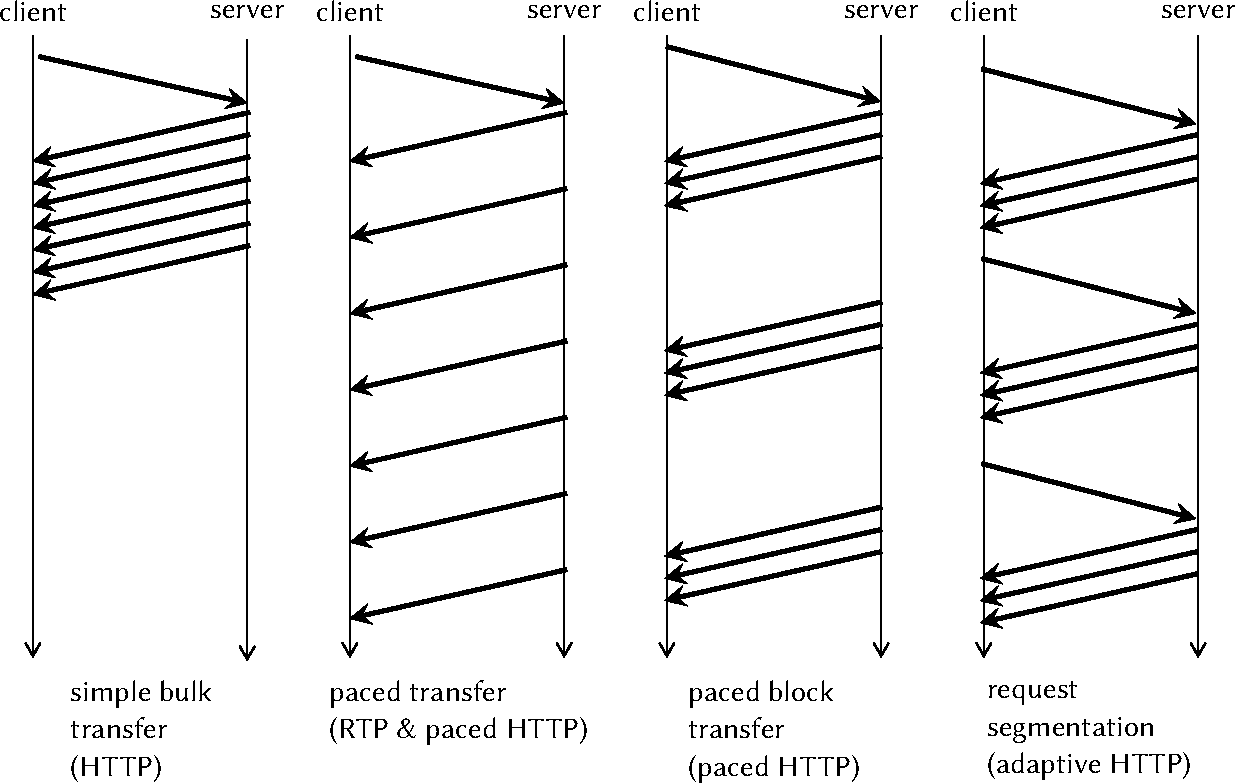
\includegraphics[width=1.0\textwidth]{images/streaming-transfer-modes.pdf}
\caption{Comparison of several possible streaming transfer modes \cite{ma2011mobile}.}
\label{c3:fig:streamingtransfermodes}
\end{figure}

\todo{reference to transmission pattern here? alternatively, put one of the old youtube throttling pictures here}

The first of the alternatives to achieve control over the playback buffer using \gls{HTTP}-streaming is to appropriately size \gls{TCP}'s flow control receive window by the application. 
Alternatively, the \gls{HTTP}-server can also manually throttle the download process, through various pacing strategies. The second and third transmission diagrams in Figure~\ref{c3:fig:streamingtransfermodes} depict two possible strategies compared to a regular \gls{HTTP} file transmission in the first transmission diagram. A third way, is to either partition the stream file into smaller even-spaced segments, that have to be requested independently, or use the aforementioned range requests on the stream's file. Through this, the receiving application can delay the request of new ranges or segments so that it matches a targeted bitrate over a longer timeframe.

These mechanism, however, can also result in a very bursty block-like transmission, a so-called ON-OFF pattern, and can cause undesirably interactions with \gls{TCP}'s flow and congestion control mechanisms \todo{ref to interaction}. Overall, stretching out the transmission may reduce server load spikes and the required buffer size on the client device but also makes streaming more vulnerable to insufficient network \gls{QoS} parameters. These specific approaches to pace to a target rate can generally be subsumed under the term \textit{Application Layer Flow Control}, which is also being implemented by some Web streaming services, e.g. YouTube \cite{alcock2011afcyt,metzger2011delivery}.

The aforementioned only adapt the transmission rate to the stream's bit rate and not the stream rate itself. Different video bitrates may be desired for many use cases, especially reacting to changing network conditions, take vertical handover from a 802.11 to a \gls{UMTS} network with a much lower throughput as an example. Quality adaptation with \gls{HTTP} streaming is generally achieved through the described range request or file segmentation mechanisms. For both approaches, multiple versions of the file or the segments have to be generated in different encoding quality levels. Also, the video file format needs to be able to support switching the stream and have an index to correlate the video files with their quality level and temporal position. \cite{ma2011mobile, watching-video1}

Several formal adaptive streaming protocols are in the process of standardization. \gls{HLS} \cite{pantos2011livestreaming} defines a playlist format to be stored separately on a server that links to all available stream variants and segments thereof in sequence. \gls{DASH} \cite{Stockhammer:2011:DAS:1943552.1943572} is a \gls{ISO}/\gls{IEC} \cite{iso-iec-23009-1} and 3GP-DASH \cite{3gpp.26.247} standard. Herein, all video segments are gathered in an alternative XML-based presentation scheme. Due to its file-based, using \gls{HTTP} for streaming is much more suited for stored video. But has also been successfully employed for live content, both \gls{HLS} as well as \gls{DASH} support this.

Other than the two streaming endpoints, the network can also, to a degree, control parts of \gls{HTTP} streaming. \gls{HTTP} allows to have forward and reverse proxies placed in the transmission's path. These could potentially alter and adapt the stream, which is however usually not done. Through \gls{DNS} video stream requests can also be redirected to a server instance chosen by the stream source. The content provider has to internally distribute the stream files to all the caches, that are advertised through \gls{DNS}. Caches are usually placed in close vicinity of potential receivers to avoid  This creates a so-called \gls{CDN} avoiding long duplicate transmission paths through the Internet and the bottleneck at a single server. \glspl{CDN} can also be used to achieve a multicast-like effect, which \gls{TCP}-based streaming cannot provide itself. Only traffic on very few links close to the recipient has to be replicated. However, the the access links of stream receivers are typically separate entities anyway, so even multicast enabeld streaming does not save bandwidth there. For an investigation of YouTube's \gls{CDN} structure refere to \cite{rafetseder2011explyt}.

Currently, \gls{HTTP} is in the process of receiving major remodeling with the efforts of WebSocket\footnote{\url{http://www.websocket.org/}} \cite{ietf2011websocket}, SPDY \cite{google2011SPDYdef,google2010SPDYwp}, and ultimately also HTTP/2.0 \cite{http20draft}. All three improve the multiplexing capabilities of \gls{HTTP} and allow the server to initiate transmissions on its own. This enables more control possibilities for the server and ca improve any segment-based adaption scheme as these segments do not need to be requested anymore but could just be pushed by the server at a convenient time.

%WebRTC \cite{webrtcdraft}


%%%%%%%%%%%%%%%%%%%%%%%%%%%%%%%%%%%%%%%%%%%%%%%%%%%%%%%%%%%%%%%%%%%%%%%%%%%%%%%%
\subsubsection{Other Approaches and Classification Matrix}

There are also other proprietary and standardized streaming systems usually tailored to specific requirements and applications. \gls{MBMS} \cite{3gpp.22.146,3gpp.22.246} is a \gls{3GPP} specification for multicasting multimedia traffic in the mobile network architecture. The explicit control structure of protocol suites like \gls{MBMS} and also \gls{IMS} \cite{3gpp.23.228} weaves application and network layer tightly together. This theoretically allows for an improved streaming performance at the cost of universally applicable behavior. \gls{RTMP} \cite{rtmpspec} is a proprietary streaming protocol which in the past has seen widespread use through its implementation in the Adobe Flash Player and Plugin in Web Browsers. Also leading a niche existence are \gls{P2P} based streaming approaches. In \gls{P2P} there is no explicit server. Instead, connections are made and stream data is exchanged between equal hosts, avoiding a centralized server's bottleneck. P2P streaming is used for example, in Tribler\footnote{\url{https://www.tribler.org/trac}} and Zattoo\footnote{\url{http://zattoo.com/int/}}.

Table~\ref{c3:tab:streamingclassification} attempts to summarize all the protocols of interest to this research and apply the proposed classification criteria to them.

\begin{table}[htb]
  \caption{Protocol Classification Matrix.}
  \label{c3:tab:streamingclassification}
  \tabulinesep=1.2mm
  \centering
  \begin{tabu}{X[0.5]XXXXXX} 
  \toprule

  \textbf{Protocol} & \textbf{Vertical Location of Control} & \textbf{Horizontal Location of Control} & \textbf{Reliable Transport} & \textbf{Video Type} & \textbf{Adaptivity} & \textbf{Multicast} \\ 
  \midrule %\tabucline[1pt]-\everyrow{\tabucline[on 1.5pt off 2pt] - }
  RTP & out-of-band application layer protocol & server-side and limited intermediary (translators and mixers) & unreliable (UDP) & low delay live streaming & server-side adaptation (transcoding) & yes, IGMP\\
  simple HTTP & in-band streaming application & client-side & reliable (TCP) & stored, not live & none & no, but emulated through CDN\\
  adaptive HTTP (DASH) & in-band streaming application & client-side & reliable (TCP) & stored and near-live & client-side with file segmentation & no, but emulated through CDN\\
  \bottomrule
  \end{tabu}
\end{table}



%%%%%%%%%%%%%%%%%%%%%%%%%%%%%%%%%%%%%%%%%%%%%%%%%%%%%%%%%%%%%%%%%%%%%%%%%%%%%%%%
%\subsubsection{Network Stack Layers and Streaming}

%In network layering models, it is often assumed that the layers are independent (or at least strongly decoupled) from, and only present narrow interfaces to, one another. From a conceptual point of view, media streaming is a process governing the application layer. Thus, the application and its behavior might be thought to dominate the overall streaming process and associated quality. In this Section, we will show that this is not necessarily the case.

%Figure \ref{c3:fig:timescales} overviews the approximate time scales on which activities on different layers may take place, spanning a remarkable range of twelve orders of magnitude. Multiple layers might implement the same or similar functionality, e.g. flow control in the application and on transport layer, resulting in nested control loops, which might be coupled due to the timing constraints. 

%\begin{figure}[htbp]
%	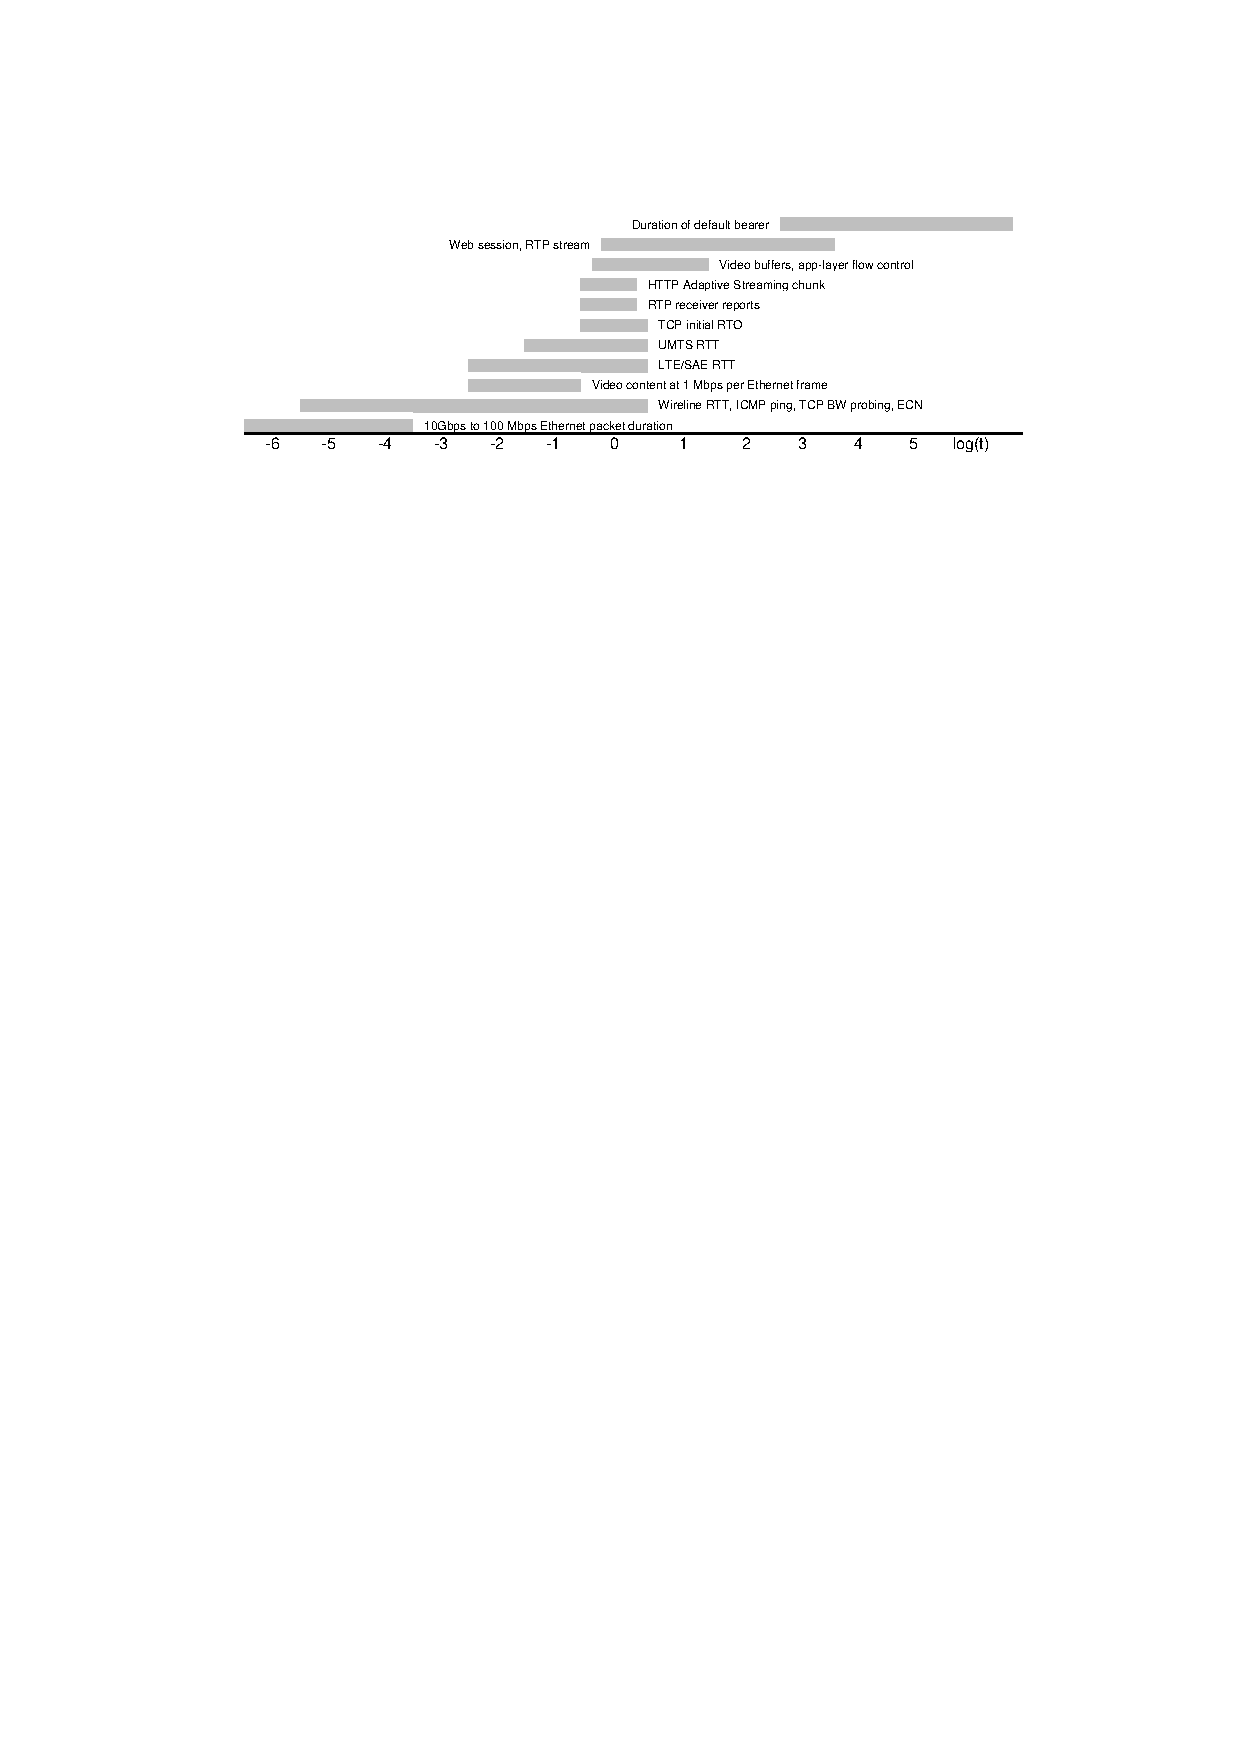
\includegraphics[width=\textwidth]{images/timescales.pdf}
%	\caption{Relevant time scales in the layers of the stack}
%	\label{c3:fig:timescales}
%\end{figure}


%\subsubsection{Network Layer}

%As seen in Figure \ref{c3:fig:timescales}, the time constants found in different network implementations range from nanoseconds (for Gigabit Ethernet) to seconds (for UMTS and \gls{LTE}/\gls{SAE} wireless networks), depending on the technology used. This also influences the achievable round-trip time across such networks, which directly affects the performance of higher-layer protocols: \gls{IP}, \gls{ICMP}, \gls{UDP}, \gls{TCP}, and subsequently all application-layer protocols are all subject to these timing constraints.

%In the case of wireless networks, typical effects of wireless connectivity relating to physical phenomena like fading and interference come into play. Flaky radio connectivity is a major source of packet loss and excessive delay. Certain cellular mobile technologies like \gls{UMTS} and its evolutions implement loss concealment themselves, confounding IP's assumption of a host-to-network layer lacking guaranteed delivery. Other peculiarities of cellular mobile networks include a \gls{MTU} opaque to IP, and delay variances as functions of packet sizes \cite{Arlos10} and radio access technologies \cite{laner2011dissecting}.


%Then, the technological progress enables both handsets and the network to become faster: Comparing the delay budgets given by x for \gls{UMTS} (2005) and y for \gls{HSDPA} R99 (2009) respectively, it is seen that the delay caused by processing on the mobile terminals decreased by a factor of 30, and that the core network has become faster by an order of magnitude as well. \cite{svoboda2006composition} has additional information on the delay budgets per network entity, varying the packet size as the parameter.



% \begin{figure}[htbp]
% \centering
% 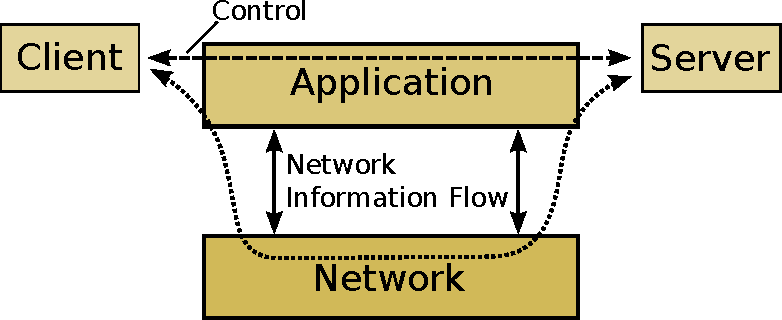
\includegraphics[width=0.8\textwidth]{images/nif.pdf}
% \caption{Theoretical information exchange paths between streaming partners.}
% \label{c3:fig:nif}
% \end{figure}

%One future trend is said to be an increase in the required communication confidentiality and authentication. One of the goals might be to enable full end-to-end encryption on the transport level of the network. This could be achieved either by providing an encrypting alternative to TCP, e.g. CurveCP \cite{curvecpwww} and TCPCrypt \cite{tcpcrypt}, or by using HTTPS and moving other functionality further up the stack.


% \subsubsection{Video Delivery Architecture}
% \label{c3:sec:videodeliveryarchitecture}
% Large Internet sites are not hosted at one central site anymore, but are usually served through geographically distributed entities forming a load-balancing structure. Such load balancing mechanisms have a long history on the Web, e.g. in the form of mirror servers a user can select manually.

% In today's Content Distribution Networks (CDN), a much larger number of mirror servers is available, and selection of a server is no longer carried out explicitly by the user, but implicitly through DNS: Content is addressed using URLs (\texttt{http://somedomain/somepath} in its simplest form), and the CDN's DNS servers are configured to resolve certain domain names to different IP addresses, depending on where the query originated.

% To get an insight into the structure of YouTube's content distribution network, we undertook a two-step measurement campaign \cite{rafetseder2011explyt}. First, we downloaded and manually parsed the HTML code served by YouTube's web servers. We could thus enumerate and learn about the structure of domain names in the system. The most relevant category of domain names for our purposes takes the form of \texttt{v$\alpha$.lscache$\beta$.c.youtube.com}, where $0<\alpha<25$ and $0<\beta<9$. Not all permutations of names are found at all times. We also noted that there are hostnames that seem to point to geographical locations, but have not succeeded so far in exhaustively mapping those two types of names.

% The second part of our campaign consisted of active measurements on forty distributed computers (part of the \textit{Seattle} Internet testbed\footnote{\url{https://seattle.poly.edu/html/}} \cite{Cappos:2009:SPE:1508865.1508905}) for over 600 hours. We learned that the frontend web server name, \texttt{www.youtube.com}, resolves to multiple IP addresses per geographical location of the probing host which are mostly disjoint from sets of addresses found on other hosts. The number of frontend IP addresses also changes over time, e.g. to account for load variations such as load increases during the evening hours in the hosts' time zones. The actual video cache servers only have one IP address per name and location each, but sometime this address is seen to change during the day. 

% When looking at the resolved addresses per frontend server and time zone, two interesting time-dependent scaling effects can be seen: First, servers become reachable or vanish in a coordinated manner controlled by the time of day, i.e. in a 24 hour pattern. We speculate this provides a gain in efficiency for the overall system to turn on parts of the resource pool for load balancing only when there is demand.

% The second type of effect occurs much more seldom. It stretches out over multiple days and is best described as follows: A new block of server IP addresses is made available in addition to the existing ones. After a few days of parallel operation, a previously active block is taken out of service. The new block continues to serve. Comparison measurements  performed in parallel show that this switch-over between IP address blocks has a positive effect on the latency to the servers, as the latency to non-YouTube destinations show no improvements at all.